\documentclass{beamer}

\mode<presentation>
{
  %\usetheme{AnnArbor}
  %\usetheme{Montpellier}
  %\usetheme{Hannover}
  %\usetheme{Singapore}
  \usetheme{Madrid}
}

\newcommand*\oldmacro{}
\let\oldmacro\insertshorttitle% ursprüngliche Definition sichern
\renewcommand*\insertshorttitle{%
  \oldmacro
  \hfill\insertframenumber\,/\,\inserttotalframenumber}

\setbeamertemplate{navigation symbols}{}

\usepackage[english]{babel}

%\usepackage[latin1]{inputenc}
\usepackage[utf8]{inputenc}

%\usepackage{hyperref}

% WTF? times? serious?
%\usepackage{times}
\usepackage[T1]{fontenc}

\usepackage{listings}

%\usepackage{tabularx}

\title[Project Proposal]{Data and Information Visualization \\ Project Proposal: MMO CombatLog Visualization}

%\subtitle {Untertitel} (optional)

\author[Brauer, Fortmann, Schmauder]
{S. Brauer \and M. Fortmann \and F. Schmauder}

\institute[UPB]{Institute for Computer Science}

\date{\today}


\subject{Computer Science}

\pgfdeclareimage[height=0.5cm]{university-logo}{upb_logo.png}
\logo{\pgfuseimage{university-logo}}



% Folgendes sollte gelöscht werden, wenn man nicht am Anfang jedes
% Unterabschnitts die Gliederung nochmal sehen möchte.
%\AtBeginSubsection[]
%{
%  \begin{frame}<beamer>{Gliederung}
%    \tableofcontents[currentsection,currentsubsection]
%  \end{frame}
%}



\begin{document}

\begin{frame}
  \titlepage
\end{frame}

\begin{frame}{The Data}
\begin{onlyenv}<1>
	\begin{itemize}
		\item CombatLog records actions from fights in the game
		\item EventBased logging
		\item Typical example of Time-Series Data
		\item Data is nominal \alert{and} quantitative
	\end{itemize}
\end{onlyenv}
\begin{onlyenv}<2>
	\begin{figure}
		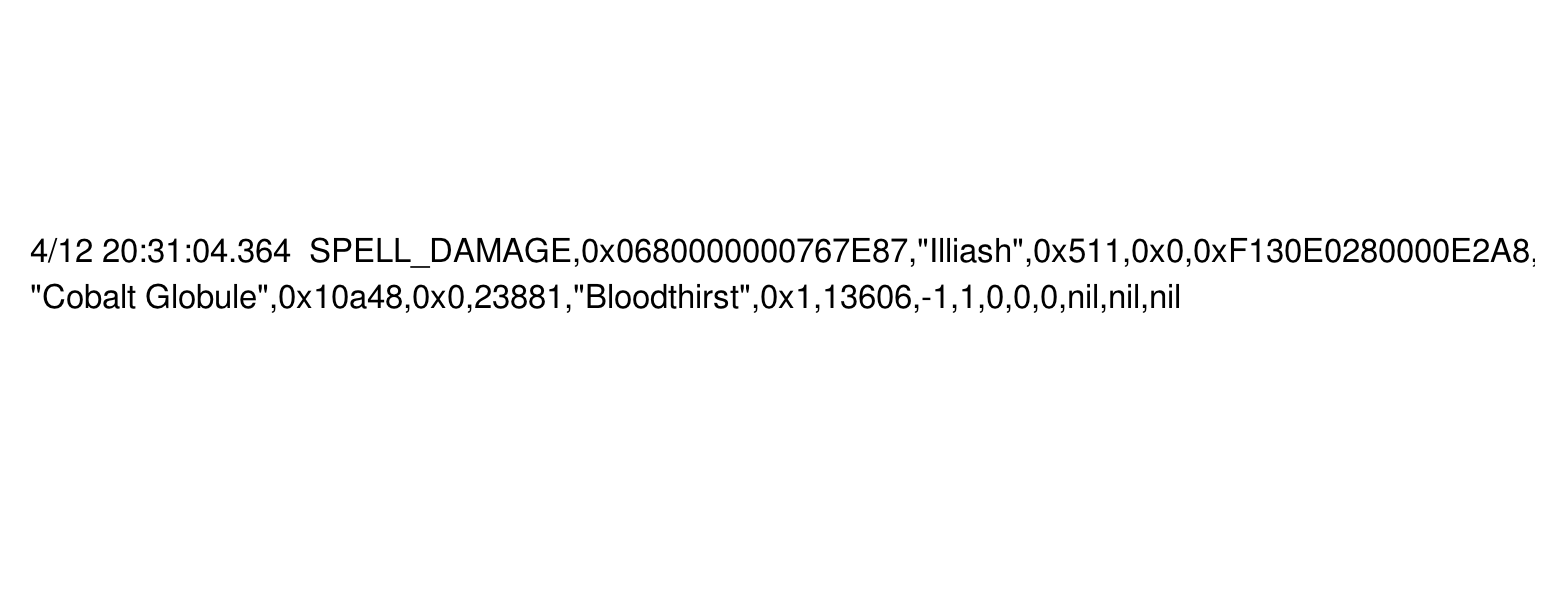
\includegraphics[width=\textwidth]{log_undecorated.png}
		\caption{Line from a CombatLog}
	\end{figure}
\end{onlyenv}
\begin{onlyenv}<3>
	\begin{figure}
		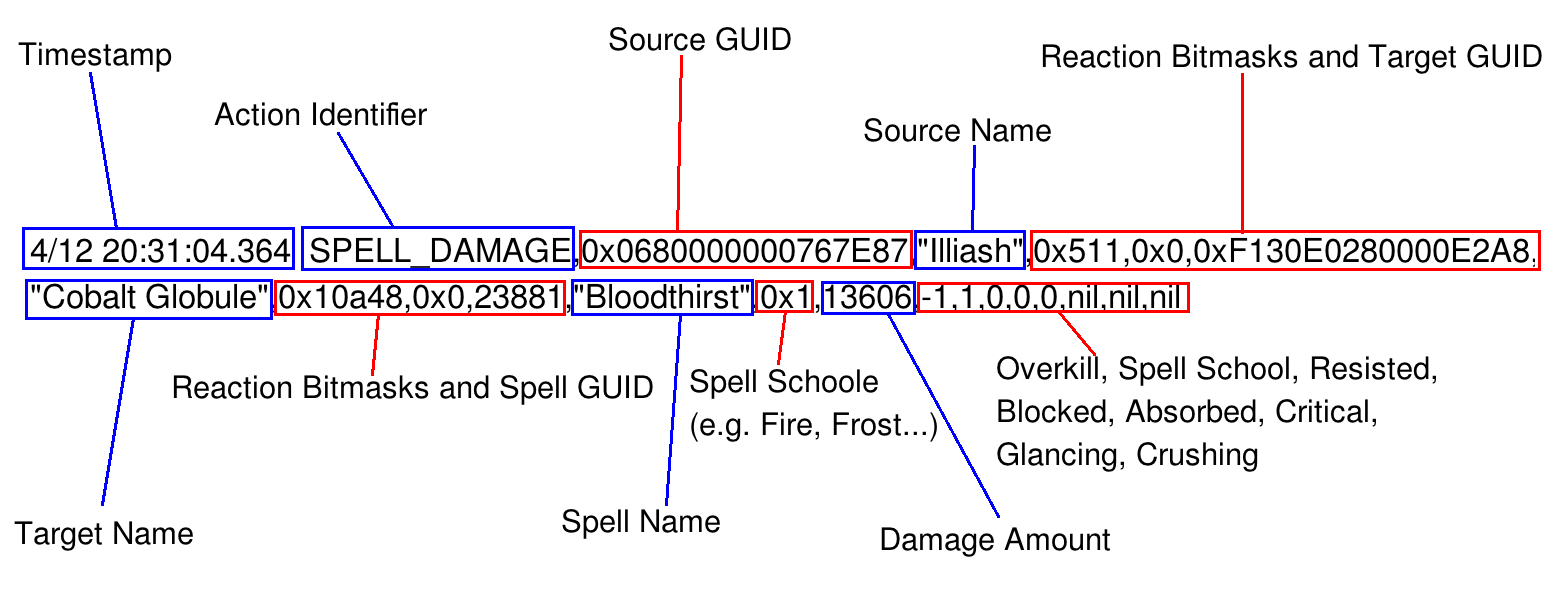
\includegraphics[width=\textwidth]{log_decorated.png}
		\caption{Line from a CombatLog}
	\end{figure}
\end{onlyenv}
\end{frame}


\begin{frame}{The User}
\begin{onlyenv}<1>
	\begin{itemize}
		\item Gamer playing a Massive Multiplayer Online Role Playing Game (MMO)
		\begin{itemize}
			\item A Member of the group recorded the log
			\item Leader of the group
			\item Any Gamer playing the specific MMORPG
		\end{itemize}
	\end{itemize}
\end{onlyenv}
\begin{onlyenv}<2>
	Visualization Goals
	\begin{itemize}
		\item Motivation
		\item Relation
		\item Improving your Performance
		\item Finding your Flaws
	\end{itemize}
\end{onlyenv}
\end{frame}


\begin{frame}{The Visualization}
\begin{onlyenv}<1>
Visualizations
\begin{itemize}
\item Line Graph
\item Pie Chart
\item Tooltips
\end{itemize}
\end{onlyenv}

\begin{onlyenv}<2>
\begin{minipage}[hbt]{0.45\textwidth}
Visualizations
\begin{itemize}
\item Line Graph
\item Pie Chart
\item Tooltips
\end{itemize}
\end{minipage}
\begin{minipage}[hbt]{0.45\textwidth}
	\begin{figure}
	\centering
	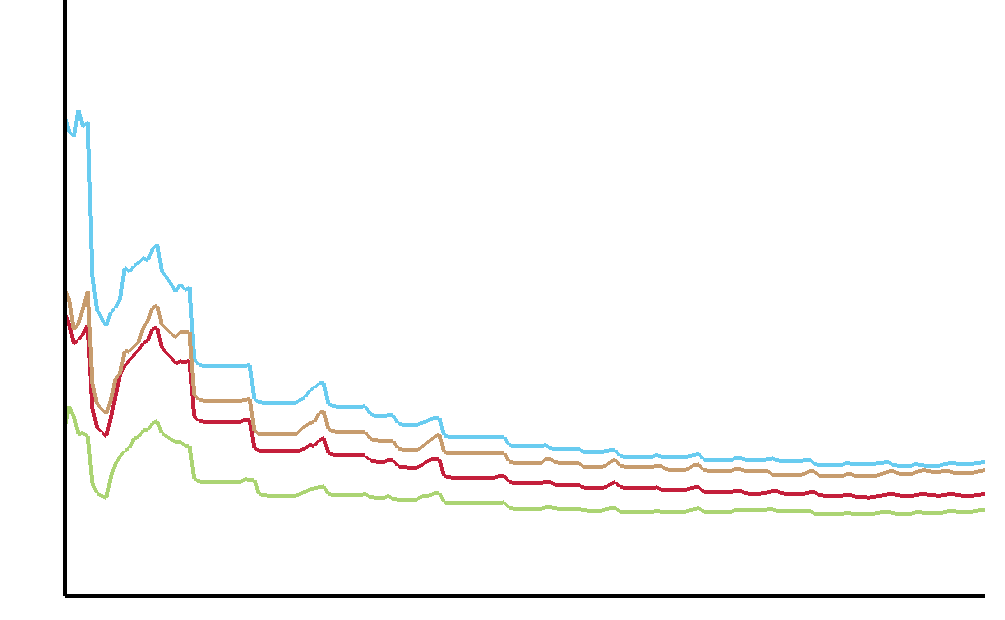
\includegraphics[width=4.5cm]{lines.png}
	\caption{Line Graph Implementation by Now}
	\end{figure}
\end{minipage}
\end{onlyenv}

\begin{onlyenv}<3>
\begin{minipage}[hbt]{0.45\textwidth}
Visualizations
\begin{itemize}
\item Line Graph
\item Pie Chart
\item Tooltips
\end{itemize}
\end{minipage}
\begin{minipage}[hbt]{0.45\textwidth}
	\begin{figure}
	\centering
	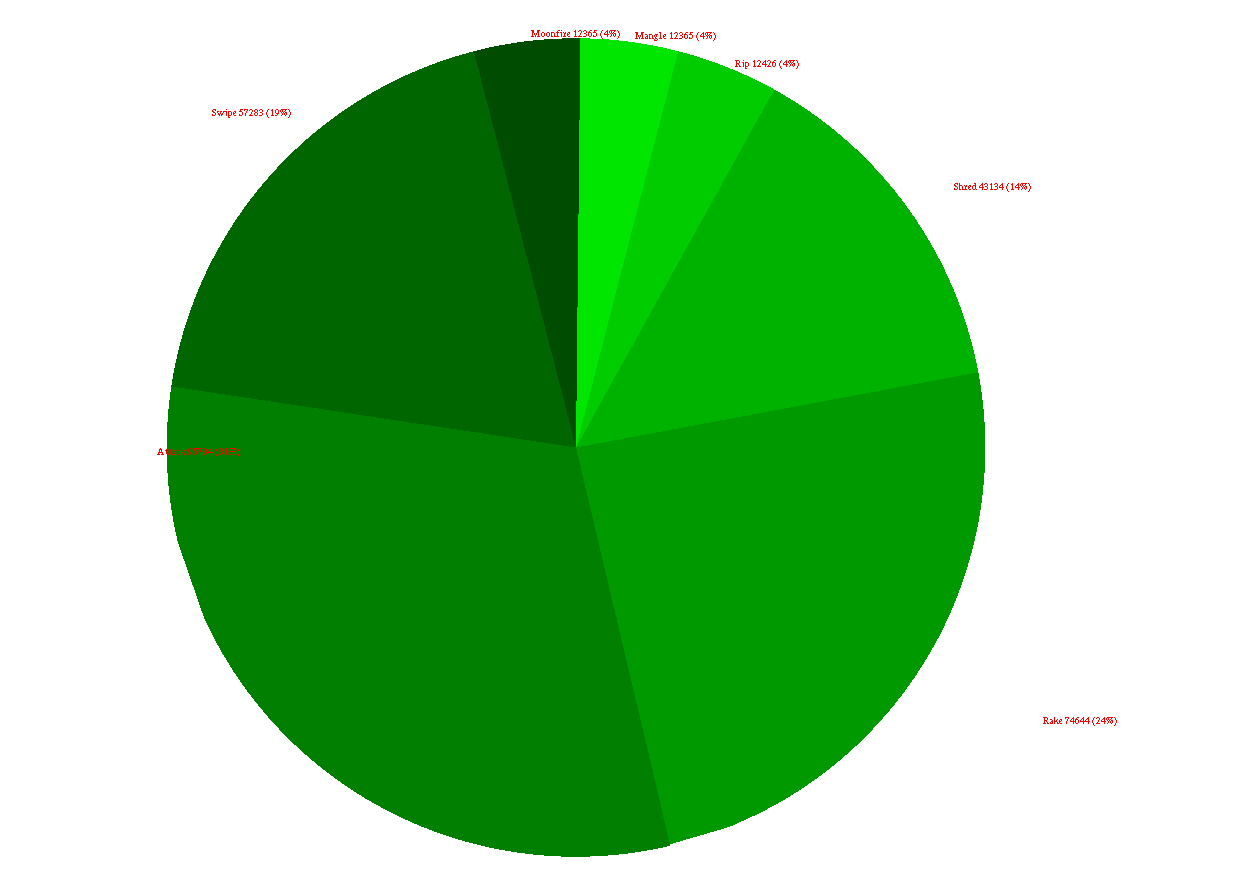
\includegraphics[width=4.5cm]{pie.png}
	\caption{Pie Chart Implementation by Now}
	\end{figure}
\end{minipage}
\end{onlyenv}

\begin{onlyenv}<4>
\begin{minipage}[hbt]{0.45\textwidth}
Visualizations
\begin{itemize}
\item Line Graph
\item Pie Chart
\item Tooltips
\end{itemize}
\end{minipage}
\begin{minipage}[hbt]{0.45\textwidth}
	\begin{figure}
	\centering
	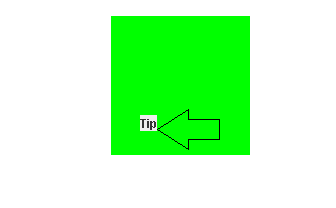
\includegraphics[width=4.5cm]{tip.png}
	\caption{Tooltip Implementation by Now}
	\end{figure}
\end{minipage}
\end{onlyenv}

\begin{onlyenv}<5>
Interaction
\begin{itemize}
\item Selective Filtering
\item Mouse Over Tooltips
\item Select and Zoom
\end{itemize}
\end{onlyenv}
\end{frame}

\end{document}
